\chapter{Реализация и экспериментальные исследования}
\label{chapter3}

В данной главе рассмотрены подробности реализации гибридного алгоритма, а также результаты экспериментов по сравнению
реализованного алгоритма с уже существующими.

Также в данной главе приведен пример задачи, использующей недоминирующую сортировку, которая использует гибридный
алгоритм, и проведено сравнение ее производительности с аналогичной реализацией задачи, использующей другой алгоритм
недоминирующей сортировки.

\section{Реализация гибридного алгоритма}

В данном разделе будут описаны подробности реализации гибридного алгоритма. Будут рассмотренны основные классы, а также
оптимизации, импользующиеся в данной реализации.

\subsection{Архитектура}

Архитектура представляет из себя абстрактный клссс, от которого наследуются три вида сорторковки. Есть абстрактный
метод, который принимает на входно input, в виде двумерного массива double, и output - массив int куда будут
записываться полученные ранги.
Важным моментом с точки зрения реализации было то, что память выделялась только в момент создания сортировщика, при
вызове на разных входных данных, с разными N и M, переиспользовались уже созданные массивы - память не выделялась снова.

\subsection{Оптимизации в алгоритме Роя}

Тут будут описаны детали реализации алгоритма Роя, которые ускоряют работу этого алгоритма, а следовательно и гибридного
алгоритма.

\subsubsection{Бинарный поиск}

В оригинальном алгоритме Роя используется линейный проход для поиска ранга для текущей вершины, но так как функция
монотонна можно использовать банарный поиск, что и было сделано. Благодаря этому алгоритм немного ускорился, хотя
асимптотика алгоритма не изменилась.

\subsection{Структуры данных}

Еще одна оптимизация, которая не меняет асимптотики алгоритма Роя, но добивается его ускорения -- использование
специальных структур данных, которые заменяют структуры, описанные в оригинальной статье.
В тратье предлагались массивы сетов и массивы сетов сетов. При реализации было принято решение заменять эти структуры
на массибы с дополнительными ссылками.
%TODO: Дописать

\section{Сравнение с существующими алгоритмами на искусственно сгенерированных тестовых данных}

В данном разделе описывается относительная эффективность работы алгоритма.

\begin{figure}
\begin{center}
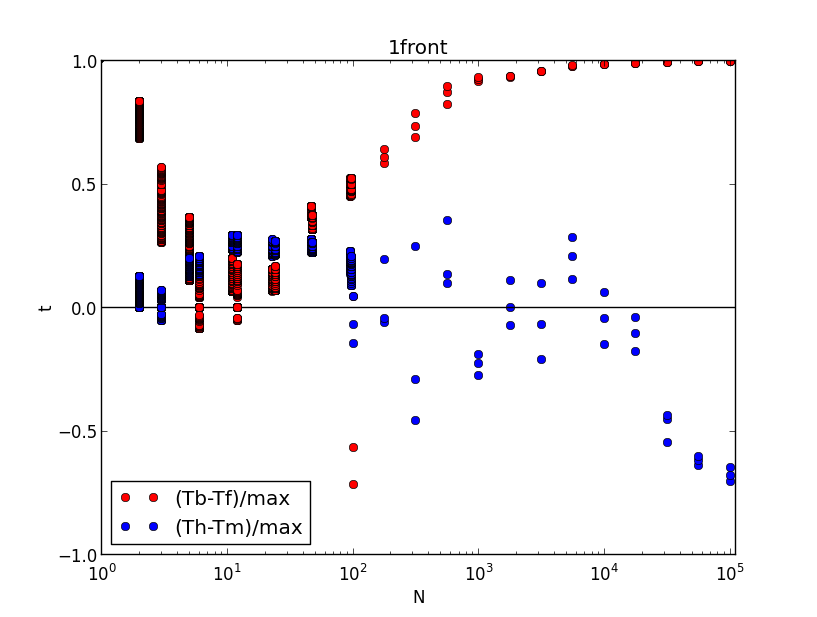
\includegraphics[width=8cm]{pic/result.png}
\caption{Относительная разность времени работы кандидатов для гибридизации в сравнении с относительной разностю времени работы с самым быстрым алгоритмом гибридного алгорима на одном из видов входных данных}
\label{experiment}
\end{center} % TODO
\end{figure}

\begin{itemize}
\item {Алгоритм работает почти так же как самый бастрый алгоритм}
\item {Начиная с некоторого n, значительно лучше}
\item {Выявлена зависимость от числа точек, размерности и фронтов}
%\item {Есть результат на реальных данных}
\end{itemize}

\section{Сравнение с существующими алгоритмами на практической задаче}

В данном разделе будет выбрана задача оптимизации, использующая наш гибридный алгоритм, и будет проведено сравнение
ее производительноси с такой же реализацией, но другим алгоритмом недоминирующей сортировки.

Была выбрана задача NSGA-II. В процессе выполнения было видно, что нас алгоритм стравляется с промежуторными
итерациями лучше, но до конца он пока что не досчитался. Авторы работы не ожидали некоторых спецэффектов реализации, о
которых не было исвестно заранее.
Пришлось запустить подсчет сначала.
Результаты будут получены в ближайщшие несколько дней.


